\documentclass[../PianoDiQualifica.tex]{subfiles}
\begin{document}
	\section{Componenti e classi principali}
		\subsection{SWEDesigner}
		I package contenuti al suo interno sono:
		\begin{itemize}
			\item SWEDesigner::Client;
			\item SWEDesigner::Server.
		\end{itemize}
		Questo package non contiene delle classi.
		\subsection{SWEDesigner::Client}
			% IMMAGINE ARCHITETTURA CLIENT GENERALE
			\begin{figure}[H]\label{fig:ClientSubsystem}
				\centering
				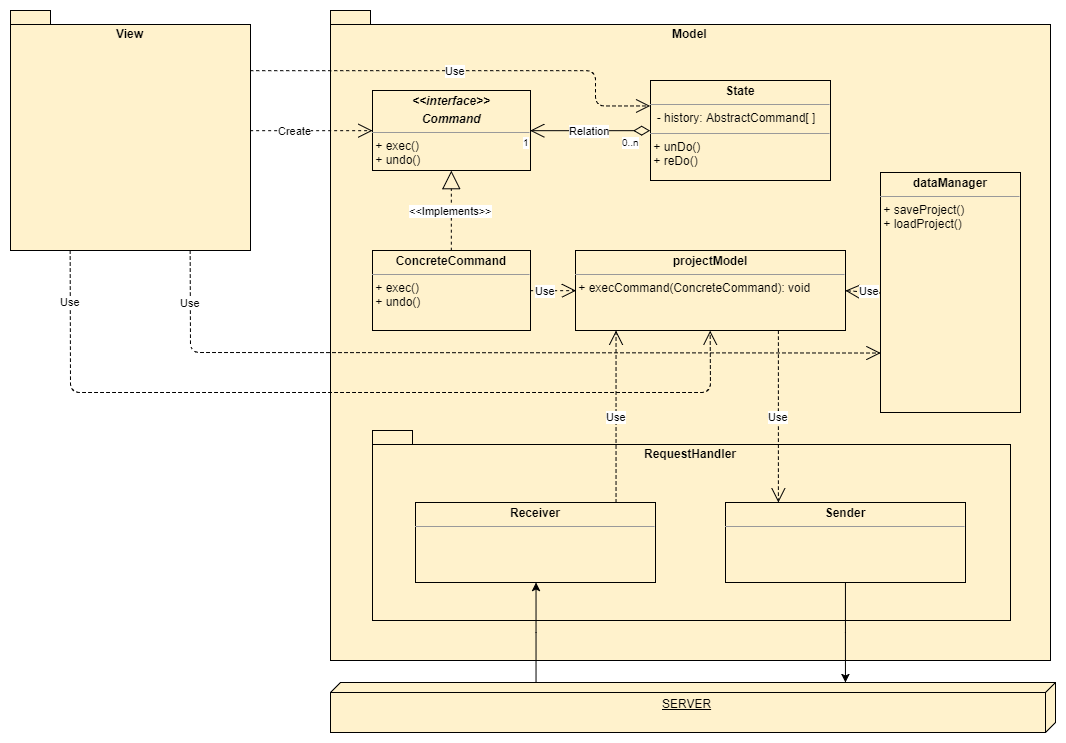
\includegraphics[scale=0.46]{Immagini/DiagrammaArchitettura/ClientSubsystem.png}
				\caption{Architettura del client}
			\end{figure}
		I package contenuti al suo interno sono:
		\begin{itemize}
			\item SWEDesigner::Client::Model;
			\item SWEDesigner::Client::View.
		\end{itemize}
		Questo package non contiene delle classi.
		\subsection{SWEDesigner::Client::Model}
		\hypertarget{SWEDesigner::Client::Model}
		I package contenuti al suo interno sono:
		\begin{itemize}
			\item SWEDesigner::Client::Model::RequestHandler.
		\end{itemize}
		Le classi contenute al suo interno verranno elencate qui di seguito.
		\subsubsection{SWEDesigner::Client::Model::Command}
		È l'interfaccia che rappresenta un generico comando impartito dai moduli View ai Model.\\
		FAN-IN:
		\begin{itemize}
			\item ConcreteCommand: implementa l'interfaccia Command per la rappresentazione concreta dei singoli comandi impartiti dai moduli View ai Model;
			\item MainView: il componente del programma che si occupa di gestire l'interfaccia grafica;
			\item State: gestisce la cronologia delle operazioni svolte permettendo le operazioni di unDo e reDo.
		\end{itemize}
		Non ci sono dipendenze OUT.
		\subsubsection{SWEDesigner::Client::Model::ConcreteCommand}
		Implementa l'interfaccia Command per la rappresentazione concreta dei singoli comandi impartiti dai moduli View ai Model.\\
		Non ci sono dipendenze IN.\\
		FAN-OUT:
		\begin{itemize}
			\item Command: è l'interfaccia che rappresenta un generico comando impartito dai moduli View ai Model;
			\item MainModel: si occupa di gestire la parte logica dell'editor.
		\end{itemize}
		\subsubsection{SWEDesigner::Client::Model::State}
		\hypertarget{SWEDesigner::Client::Model::State}
		Gestisce la cronologia delle operazioni svolte permettendo le operazioni di unDo e reDo.\\
		FAN-IN:
		\begin{itemize}
			\item MainView: il componente del programma che si occupa di gestire l'interfaccia grafica.
		\end{itemize}
		FAN-OUT:
		\begin{itemize}
			\item Command: è l'interfaccia che rappresenta un generico comando impartito dai moduli View ai Model.
		\end{itemize}.
		\subsubsection{SWEDesigner::Client::Model::DAO}
		\hypertarget{SWEDesigner::Client::Model::DAO}
		Si occupa della persistenza dei dati, in particolare del salvataggio su file system locale del progetto già esistente.\\
		FAN-IN:
		\begin{itemize}
			\item MainView: il componente del programma che si occupa di gestire l'interfaccia grafica.
		\end{itemize}
		FAN-OUT:
		\begin{itemize}
			\item MainModel: si occupa di gestire la parte logica dell'editor.
		\end{itemize}
		\subsubsection{SWEDesigner::Client::Model::MainModel}
			% IMMAGINE ARCHITETTURA MAINMODEL
			\begin{figure}[H]\label{fig:MainModel}
				\centering
				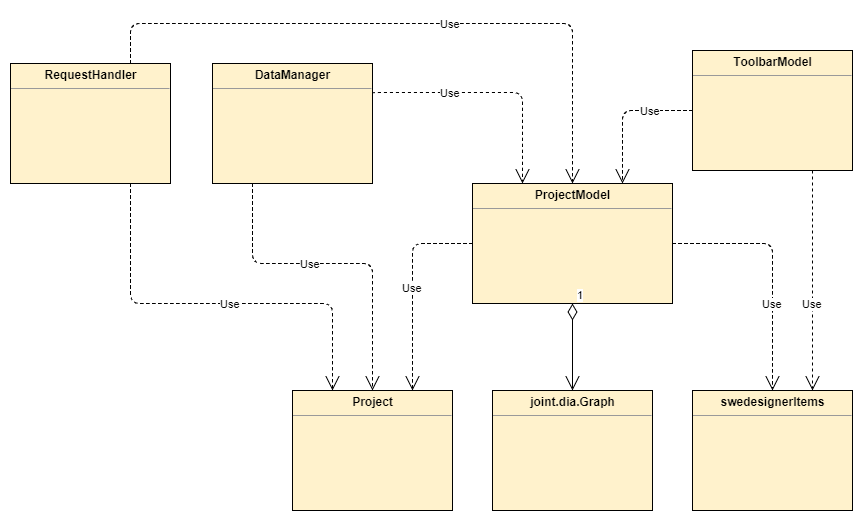
\includegraphics[scale=0.46]{Immagini/DiagrammaArchitettura/MainModel.png}
				\caption{Architettura di MainModel}
			\end{figure}
		È il componente del programma che si occupa di gestire la parte logica dell’editor.\\
		FAN-IN:
		\begin{itemize}
			\item ConcreteCommand: rappresenta i comandi inviati dalle View ed eseguiti poi da Model;
			\item DAO: si occupa della persistenza dei dati, in particolare del salvataggio su file system locale del progetto e del caricamento di un progetto già esistente;
			\item MainView: invoca il metodo execCommand;
			\item Client::RequestHandler::Receiver: si occupa di gestire i dati ricevuti dal server.
		\end{itemize}
		FAN-OUT:
		\begin{itemize}
			%\item Client::Model::TitleBarModel: declina le funzionalità di model per la barra del titolo;
			%\item Client::Model::ToolBarModel: declina le funzionalità di model per la toolbar laterale;
			%\item Client::Model::AddressModel: declina le funzionalità di model per la barra di indirizzo;
			%\item Client::Model::EditPanelModel: declina le funzionalità di model per il pannello di editing laterale;
			%\item Client::Model::DiagramTree: è la collezione di tutti i model associati a ciascun diagramma;
			\item Client::RequestHandler::Sender: si occupa di gestire le comunicazioni in uscita verso il server.
		\end{itemize}
		\subsubsection{SWEDesigner::Client::Model::TitleBarModel}
		\hypertarget{SWEDesigner::Client::Model::TitleBarModel}
		Si occupa di gestire la parte logica della barra del titolo.\\
		FAN-IN:
		\begin{itemize}
			\item MainModel: si occupa di gestire la parte logica dell'editor.
		\end{itemize}
		Non ci sono dipendenze OUT.
		\subsubsection{SWEDesigner::Client::Model::ToolBarModel}
		È il componente del programma che si occupa di gestire la parte logica delle toolbar.\\
		FAN-IN:
		\begin{itemize}
			\item MainModel: si occupa di gestire la parte logica dell'editor;
			\item PackageToolbar: rappresenta la particolare toolbar legata all'editor del diagramma dei package;
			\item ClassToolbar: rappresenta la particolare toolbar legata all'editor del diagramma delle classi;
			\item ActivityToolbar: rappresenta la particolare toolbar legata all'editor del diagramma delle attività;
			\item BubbleToolbar: rappresenta la particolare toolbar legata all'editor del bubble flowchart.
		\end{itemize}
		Non ci sono dipendenze OUT.
		\subsubsection{SWEDesigner::Client::Model::PackageToolbar}
		\hypertarget{SWEDesigner::Client::Model::PackageToolbar}
		Rappresenta la particolare toolbar legata all’editor del diagramma dei package.\\
		Non ci sono dipendenze IN.\\
		FAN-OUT:
		\begin{itemize}
			\item ToolbarModel: è il componente del programma che si occupa di gestire la parte logica delle toolbar.
		\end{itemize}
		\subsubsection{SWEDesigner::Client::Model::ClassToolbar}
		\hypertarget{SWEDesigner::Client::Model::ClassToolbar}
		Rappresenta la particolare toolbar legata all’editor del diagramma delle classi.\\
		Non ci sono dipendenze IN.\\
		FAN-OUT:
		\begin{itemize}
			\item ToolbarModel: è il componente del programma che si occupa di gestire la parte logica delle toolbar.
		\end{itemize}
		\subsubsection{SWEDesigner::Client::Model::ActivityToolbar}
		\hypertarget{SWEDesigner::Client::Model::ActivityToolbar}
		Rappresenta la particolare toolbar legata all’editor del diagramma delle attività.\\
		Non ci sono dipendenze IN.\\
		FAN-OUT:
		\begin{itemize}
			\item ToolbarModel: è il componente del programma che si occupa di gestire la parte logica delle toolbar.
		\end{itemize}
		\subsubsection{SWEDesigner::Client::Model::BubbleToolbar}
		\hypertarget{SWEDesigner::Client::Model::BubbleToolbar}
		Rappresenta la particolare toolbar legata all’editor del bubble flowchart.\\
		Non ci sono dipendenze IN.\\
		FAN-OUT:
		\begin{itemize}
			\item ToolbarModel: è il componente del programma che si occupa di gestire la parte logica delle toolbar.
		\end{itemize}
		\subsubsection{SWEDesigner::Client::Model::AddressModel}
		\hypertarget{SWEDesigner::Client::Model::AddressModel}
		Si occupa di gestire la parte logica della barra degli indirizzi.\\
		FAN-IN:
		\begin{itemize}
			\item MainModel: si occupa di gestire la parte logica dell'editor.
		\end{itemize}
		Non ci sono dipendenze OUT.
		\subsubsection{SWEDesigner::Client::Model::EditPanelModel}
		\hypertarget{SWEDesigner::Client::Model::EditPanelModel}
		Si occupa di gestire la parte logica del pannello di editing laterale.\\
		FAN-IN:
		\begin{itemize}
			\item ItemPanel: estende la funzionalità di editPanelModel specificamente per ciascun oggetto selezionato;
			\item MainModel: si occupa di gestire la parte logica dell'editor.
		\end{itemize}
		Non ci sono dipendenze OUT.\\
		\subsubsection{SWEDesigner::Client::Model::ItemPanel}
		Estende la funzionalità di EditPanelModel specificamente per ciascun oggetto selezionato.\\
		Non ci sono dipendenze IN.\\
		FAN-OUT:
		\begin{itemize}
			\item EditPanelModel: si occupa di gestire la parte logica del pannello di editing laterale.
		\end{itemize}
		\subsubsection{SWEDesigner::Client::Model::DiagramTree}
		È la collezione di tutti i model associati a ciascun diagramma.\\
		FAN-IN:
		\begin{itemize}
			\item MainModel: si occupa di gestire la parte logica dell'editor.
		\end{itemize}
		FAN-OUT:
		\begin{itemize}
			\item Diagram: si occupa di gestire la parte logica di un diagramma.
		\end{itemize}
		\subsubsection{SWEDesigner::Client::Model::Diagram}
		Si occupa di gestire la parte logica di un diagramma.\\
		FAN-IN:
		\begin{itemize}
			\item ActivityDiagram: estenda la funzionalità di Diagram per rappresentare un diagramma delle attività;
			\item BubbleDiagram: estende la funzionalità di Diagram per rappresentare un bubble flowchart;
			\item ClassDiagram: estende la funzionalità di Diagram per rappresentare un diagramma delle classi;
			\item DiagramTree: è la collezione di tutti i model associati a ciascun diagramma;
			\item PackageDiagram: estende la funzionalità di Diagram per rappresentare un diagramma dei package.
		\end{itemize}
		FAN-OUT:
		\begin{itemize}
			\item joint.dia.Graph: fa la funzione di model all'interno della libreria grafica JoinJS.
		\end{itemize}
		\subsubsection{SWEDesigner::Client::Model::PackageDiagram}
		\hypertarget{SWEDesigner::Client::Model::PackageDiagram}
		Estende le funzionalità di Diagram per rappresentare un diagramma dei package.\\
		Non ci sono dipendenze IN.\\
		FAN-OUT:
		\begin{itemize}
			\item Diagram: si occupa di gestire la parte logica di un diagramma.
		\end{itemize}
		\subsubsection{SWEDesigner::Client::Model::ClassDiagram}
		\hypertarget{SWEDesigner::Client::Model::ClassDiagram}
		Estende le funzionalità di Diagram per rappresentare un diagramma delle classi.\\
		Non ci sono dipendenze IN.\\
		FAN-OUT:
		\begin{itemize}
			\item Diagram: si occupa di gestire la parte logica di un diagramma.
		\end{itemize}
		\subsubsection{SWEDesigner::Client::Model::ActivityDiagram}
		\hypertarget{SWEDesigner::Client::Model::ActivityDiagram}
		Estende le funzionalità di Diagram per rappresentare un diagramma delle attività.\\
		Non ci sono dipendenze IN.\\
		FAN-OUT:
		\begin{itemize}
			\item Diagram: si occupa di gestire la parte logica di un diagramma.
		\end{itemize}
		\subsubsection{SWEDesigner::Client::Model::BubbleDiagram}
		\hypertarget{SWEDesigner::Client::Model::BubbleDiagram}
		Estende le funzionalità di Diagram per rappresentare un bubble flowchart.\\
		Non ci sono dipendenze IN.\\
		FAN-OUT:
		\begin{itemize}
			\item Diagram: si occupa di gestire la parte logica di un diagramma.
		\end{itemize}
		\subsection{SWEDesigner::Client::Model::RequestHandler}
		\hypertarget{SWEDesigner::Client::Model::RequestHandler}
		Questo package non contiene dei sottopackage.\\
		Le classi contenute al suo interno verranno elencate qui di seguito.
		\subsubsection{SWEDesigner::Client::Model::RequestHandler::Sender}
		Si occupa di gestire le comunicazioni in uscita verso il server.\\
		FAN-IN:
		\begin{itemize}
			\item MainModel: si occupa di gestire la parte logica dell'editor.
		\end{itemize}
		FAN-OUT:
		\begin{itemize}
			\item Server::RequestHandler::Receiver: si occupa di gestire le comunicazioni in entrata dal Client.
		\end{itemize}
		\subsubsection{SWEDesigner::Client::Model::RequestHandler::Receiver}
		Si occupa di gestire le comunicazioni in entrata dal server.\\
		FAN-IN:
		\begin{itemize}
			\item Server::RequestHandler::Sender: si occupa di gestire le comunicazioni in uscita verso il Client.
		\end{itemize}
		FAN-OUT:
		\begin{itemize}
			\item MainModel: si occupa di gestire la parte logica dell'editor.
		\end{itemize}
		\subsection{SWEDesigner::Client::View}
		\hypertarget{SWEDesigner::Client::View}
		Questo package non contiene dei sottopackage.
		Le classi contenute al suo interno verranno elencate qui di seguito.
		\subsubsection{SWEDesigner::Client::View::MainView}
			% IMMAGINE ARCHITETTURA MAINVIEW
			\begin{figure}[H]\label{fig:MainModel}
				\centering
				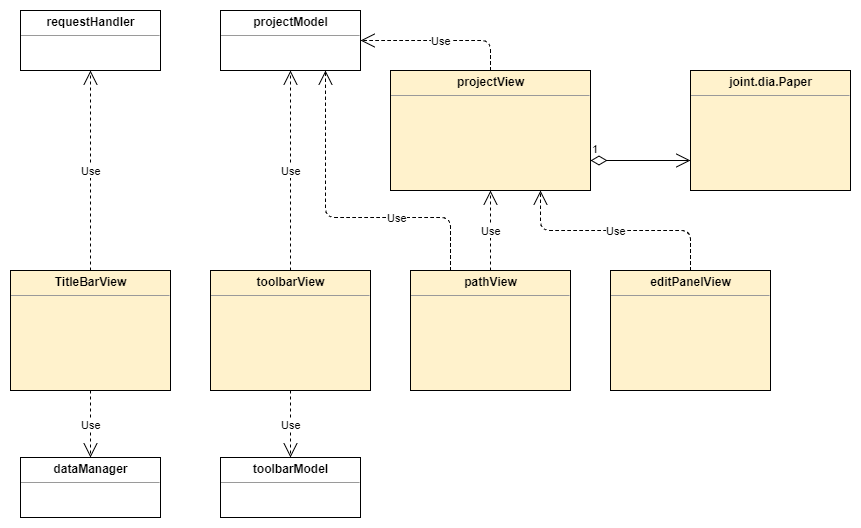
\includegraphics[scale=0.44]{Immagini/DiagrammaArchitettura/MainView.png}
				\caption{Architettura di MainView}
			\end{figure}
		È il componente del programma che si occupa di gestire l'interfaccia grafica. Nella particolare declinazione MVC adottata da Backbone.js, si occupa anche di gestire gli input dell'utente e si interfaccia con il model attraverso dei command. È un aggregatore di altre classi View specializzate nella gestione dei diversi elementi dell'interfaccia grafica, in particolare TitleBarView, ToolBarView, AddressView, EditPanelView e Paper.\\
		Non ci sono dipendenze IN.\\
			FAN-OUT:
			\begin{itemize}
				\item State: si occupa di gestire la cronologia delle operazioni svolte;
				\item DAO: si occupa di gestire la persistenza dei dati;
				\item MainModel: si occupa di gestire la parte logica dell'editor;
				\item Command: rappresenta un comando generico impartito dai moduli View ai Model;
				\item TitleBarView: gestisce l'interfaccia grafica della barra del titolo;
				\item ToolbarView: gestisce l'interfaccia grafica della barra degli strumenti;
				\item AddressView: gestisce l'interfaccia grafica della barra di indirizzo;
				\item EditPanelView: gestisce l'interfaccia grafica del pannello di editing;
				\item Paper: gestisce l'interfaccia grafica dell'area dei diagrammi.
			\end{itemize}
		\subsubsection{SWEDesigner::Client::View::TitleBarView}
		È il componente del programma che fa la funzione di view per la barra del titolo, dove saranno collocati il menu dell’applicazione e gli shortcut.\\
		FAN-IN:
		\begin{itemize}
			\item MainView: si occupa di gestire la parte grafica del model.
		\end{itemize}
		Non ci sono dipendenze OUT.\\
		%FAN-OUT:
		%\begin{itemize}
		%	\item TitleBarModel: declina le funzionalità di model per la barra del titolo.
		%\end{itemize}
		\subsubsection{SWEDesigner::Client::View::ToolBarView}
		È il componente del programma che fa la funzione di view per la toolbar dove saranno collocati gli strumenti per editare i diagrammi.\\
		FAN-IN:
		\begin{itemize}
			\item MainView: si occupa di gestire la parte grafica del model.
		\end{itemize}
		Non ci sono dipendenze OUT.\\
		%FAN-OUT:
		%\begin{itemize}
		%	\item ToolBarModel: declina le funzionalità di model per la barra degli strumenti.
		%\end{itemize}
		\subsubsection{SWEDesigner::Client::View::AddressView}
		È il componente del programma che fa la funzione di view per il cosiddetto breadcrumb dove viene inserita la posizione corrente.\\
		FAN-IN:
		\begin{itemize}
			\item MainView: si occupa di gestire la parte grafica del model.
		\end{itemize}
		Non ci sono dipendenze OUT.\\
		%FAN-OUT:
		%\begin{itemize}
		%	\item AddressModel: declina le funzionalità di model per la barra di indirizzo.
		%\end{itemize}
		\subsubsection{SWEDesigner::Client::View::EditPanelView}
		È il componente del programma che fa la funzione di view per le informazioni editabili degli elementi che fanno parte dei diversi diagrammi.\\
		FAN-IN:
		\begin{itemize}
			\item MainView: si occupa di gestire la parte grafica del model.
		\end{itemize}
		Non ci sono dipendenze OUT.\\
		%FAN-OUT:
		%\begin{itemize}
		%	\item EditPanelModel: declina le funzionalità di model per il pannello di editing laterale.
		%\end{itemize}
		\subsubsection{SWEDesigner::Client::View::Paper}
		È il componente del programma che fa la funzione di view per i diversi diagrammi.\\
		FAN-IN:
		\begin{itemize}
			\item MainView: si occupa di gestire la parte grafica del model.
		\end{itemize}
		FAN-OUT:
		\begin{itemize}
			%\item Diagram: si occupa di gestire la parte logica di un diagramma;
			\item joint.dia.Paper: classe che rappresenta la View dei diagrammi all'interno della libreria grafica JointJS.
		\end{itemize}
		\subsection{SWEDesigner::Server}
			% IMMAGINE ARCHITETTURA SERVER GENERALE
			\begin{figure}[H]\label{fig:ServerSubsystem}
				\centering
				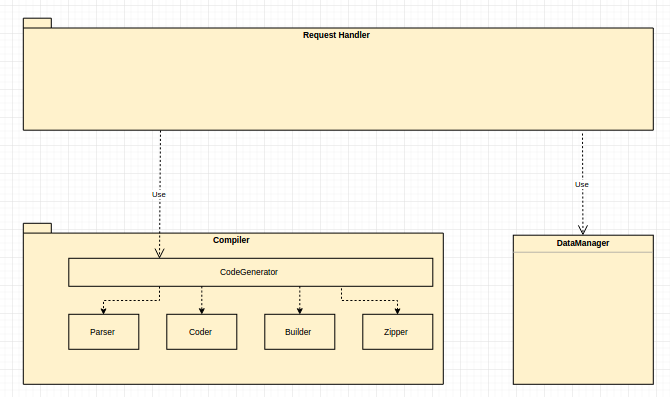
\includegraphics[scale=0.4]{Immagini/DiagrammaArchitettura/ServerSubsystem.png}
				\caption{Architettura del server}
			\end{figure}
		I package contenuti al suo interno sono:
		\begin{itemize}
			\item SWEDesigner::Server::CodeGenerator;
			\item SWEDesigner::Server::DAORequestHandler;
			\item SWEDesigner::Server::RequestHandler.
		\end{itemize}
		Questo package non contiene delle classi.
		\subsection{SWEDesigner::Server::CodeGenerator}
		I package contenuti al suo interno sono:
		\begin{itemize}
			\item SWEDesigner::Server::CodeGenerator::Builder;
			\item SWEDesigner::Server::CodeGenerator::Coder;
			\item SWEDesigner::Server::CodeGenerator::Parser;
			\item SWEDesigner::Server::CodeGenerator::Zipper.
		\end{itemize}
		Le classi contenute al suo interno verranno elencate qui di seguito.
		\subsubsection{SWEDesigner::Server::CodeGenerator::CodeGenerator}
		\hypertarget{SWEDesigner::Server::CodeGenerator::CodeGenerator}
		E' il componente che rende disponibile la funzionalità per cui, dato un file valido in formato JSON, restituisce un pacchetto in formato .zip contenente i file del codice sorgente che costituiscono il programma rappresentato dal file in input. I file prodotti sono strutturati in packages, come indicato nel file JSON in input.\\
		FAN-IN:
		\begin{itemize}
			\item Server::RequestHandler::Receiver: si occupa di gestire le comunicazioni in entrata dal client.
		\end{itemize}
			FAN-OUT:
			\begin{itemize}
				\item Server::RequestHandler::Sender: si occupa di gestire le comunicazioni in uscita verso il client;
				\item Parser: si occupa di creare un oggetto che contiene le informazioni ricevute in input;
				\item Zipper: si occupa di creare un archivio .zip contenente in codici sorgente precedentemente creati.
			\end{itemize}
		\subsection{SWEDesigner::Server::CodeGenerator::Builder}
		Questo package non contiene dei sottopackage.\\
		Le classi contenute al suo interno verranno elencate qui di seguito.
		\subsubsection{SWEDesigner::Server::CodeGenerator::Builder::Builder}
		È il componente che rende disponibile la funzionalità, dato un file JSON in input che rappresenti un programma, di ottenere un oggetto contenitore del codice sorgente corrispondente al contenuto del file di input. Tale codice è suddiviso e strutturato come indicato nel file di input.\\
			FAN-IN:
			\begin{itemize}
				\item Zipper: si occupa di creare un archivio .zip contenente in codici sorgente precedentemente creati.
			\end{itemize}
			FAN-OUT:
			\begin{itemize}
				\item Coder: componente che funge da interfaccia alle operazioni di codifica di una stringa permettendo quindi di trasformare le informazioni del file in formato JSON in codice sorgente.
			\end{itemize}
		\subsection{SWEDesigner::Server::CodeGenerator::Coder}
			% IMMAGINE ARCHITETTURA CODER
			\begin{figure}[H]\label{fig:Coder}
				\centering
				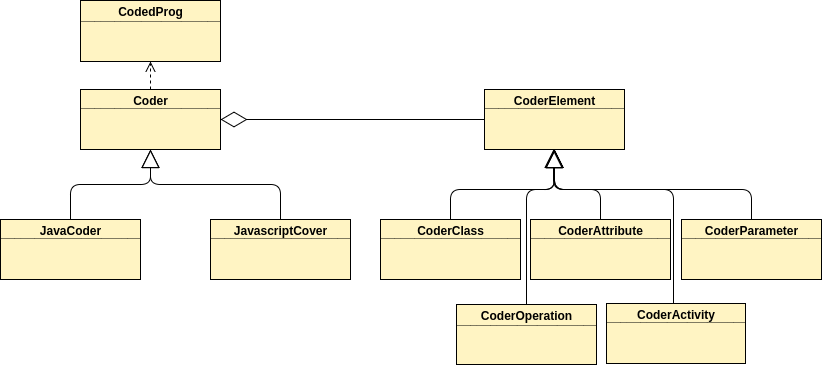
\includegraphics[scale=0.46]{Immagini/DiagrammaArchitettura/Coder.png}
				\caption{Architettura di Coder}
			\end{figure}
		Questo package non contiene dei sottopackage.\\
		Le classi contenute al suo interno verranno elencate qui di seguito.
		\subsubsection{SWEDesigner::Server::CodeGenerator::Coder::Coder}
		Componente che funge da interfaccia alle operazioni di codifica di una stringa, in formato JSON che rappresenta un programma valido; tali operazioni permettono di ottenere un oggetto contenente il codice sorgente, in Java o Javascript, corrispondente alla stringa in input.\\
		FAN-IN:
		\begin{itemize}
			\item JavaCoder: si occupa di trasformare un oggetto JSON ricevuto in input in un oggetto contenente il codice sorgente scritto in java;
			\item JavaScriptCoder: si occupa di trasformare un oggetto JSON ricevuto in input in un oggetto contenente il codice sorgente scritto in javascript.
		\end{itemize}
		FAN-OUT:
		\begin{itemize}
			\item CodedProg: componente che contiene il codice prodotto dal Coder;
			\item CoderElement: componente astratto che offre la funzionalità che permette di associare ad ogni stringa contenuta nel file JSON il corrispondente codice sorgente.
		\end{itemize}
		\subsubsection{SWEDesigner::Server::CodeGenerator::Coder::JavaCoder}
		È il componente che rende disponibile la funzionalità, dato un oggetto in input che rappresenta un file JSON parsificato, di ottenere un oggetto contenente il codice sorgente, in linguaggio Java, corrispondente all'oggetto in input.\\
		Non ci sono dipendenze IN.\\
			FAN-OUT:
			\begin{itemize}
				\item Coder: componente che funge da interfaccia alle operazioni di codifica di una stringa permettendo quindi di trasformare le informazioni del file in formato JSON in codice sorgente.
			\end{itemize}
		\subsubsection{SWEDesigner::Server::CodeGenerator::Coder::JavascriptCoder}
		È il componente che rende disponibile la funzionalità, dato un oggetto in input che rappresenta un file JSON parsificato, di ottenere un oggetto contenente il codice sorgente, in linguaggio Javascript, corrispondente all'oggetto in input.\\
		Non ci sono dipendenze IN.\\
		FAN-OUT:
		\begin{itemize}
			\item Coder: componente che funge da interfaccia alle operazioni di codifica di una stringa permettendo quindi di trasformare le informazioni del file in formato JSON in codice sorgente.
		\end{itemize}
		\subsubsection{SWEDesigner::Server::CodeGenerator::Coder::CoderClass}
		È il componente che mette a disposizione la funzionalità, data una stringa in input in formato JSON che rappresenta una classe valida, di ottenere il corrispondente codice sorgente di tale classe.\\
		Non ci sono dipendenze IN.\\
	FAN-OUT:
	\begin{itemize}
		\item CoderElement: componente astratto che offre la funzionalità che permette di associare ad ogni stringa contenuta nel file JSON il corrispondente codice sorgente.
	\end{itemize}
		\subsubsection{SWEDesigner::Server::CodeGenerator::Coder::CoderOperation}
		È il componente che mette a disposizione la funzionalità, data una stringa in input in formato JSON che rappresenta un'operazione valida, di ottenere il corrispondente codice sorgente di tale operazione.\\
		Non ci sono dipendenze IN.\\
		FAN-OUT:
		\begin{itemize}
			\item CoderElement: componente astratto che offre la funzionalità che permette di associare ad ogni stringa contenuta nel file JSON il corrispondente codice sorgente.
		\end{itemize}
		\subsubsection{SWEDesigner::Server::CodeGenerator::Coder::CoderParameter}
		È il componente che mette a disposizione la funzionalità, data una stringa in input in formato JSON che rappresenta un parametro di una lista valido, di ottenere il corrispondente codice sorgente di tale parametro. È possibile scegliere fra la codifica in Java o Javascript.\\
		Non ci sono dipendenze IN.\\
		FAN-OUT:
		\begin{itemize}
			\item CoderElement: componente astratto che offre la funzionalità che permette di associare ad ogni stringa contenuta nel file JSON il corrispondente codice sorgente.
		\end{itemize}
			\subsubsection{SWEDesigner::Server::CodeGenerator::Coder::CoderAttribute}
			È il componente che mette a disposizione la funzionalità, data una stringa in input in formato JSON che rappresenta un attributo valido, di ottenere il corrispondente codice sorgente di tale attributo. È possibile scegliere fra la codifica in Java o Javascript.\\
			Non ci sono dipendenze IN.\\
			FAN-OUT:
			\begin{itemize}
				\item CoderElement: componente astratto che offre la funzionalità che permette di associare ad ogni stringa contenuta nel file JSON il corrispondente codice sorgente.
			\end{itemize}
		\subsubsection{SWEDesigner::Server::CodeGenerator::Coder::CoderActivity}
		È il componente che mette a disposizione la funzionalità, data una stringa in input in formato JSON che rappresenta un diagramma delle attività valido, di ottenere il corrispondente codice sorgente di tale attività. È possibile scegliere fra la codifica in Java o Javascript.\\
		Non ci sono dipendenze IN.\\
		FAN-OUT:
		\begin{itemize}
			\item CoderElement: componente astratto che offre la funzionalità che permette di associare ad ogni stringa contenuta nel file JSON il corrispondente codice sorgente;
			\item DAO: si occupa di gestire il database delle bubble.
		\end{itemize}
		\subsubsection{SWEDesigner::Server::CodeGenerator::Coder::CodedProg}
		È il componente che contiene il codice sorgente prodotto dal Coder.\\
		FAN-IN:
		\begin{itemize}
			\item Coder: componente che funge da interfaccia alle operazioni di codifica di una stringa permettendo quindi di trasformare le informazioni del file in formato JSON in codice sorgente.
		\end{itemize}
		Non ci sono dipendenze OUT.
		
		\subsubsection{SWEDesigner::Server::CodeGenerator::Coder::CoderElement}
		Componente astratta che offre la funzionalità di ottenere, data una stringa in input in formato JSON che rappresenta un elemento di classe valido, il corrispondente codice sorgente, in Java o Javascript.\\
		FAN-IN:
		\begin{itemize}
			\item Coder: componente che funge da interfaccia alle operazioni di codifica di una stringa permettendo quindi di trasformare le informazioni del file in formato JSON in codice sorgente;
			\item CoderClass: componente che permette data una stringa in input in formato JSON che rappresenta un diagramma delle classi valido, di ottenere il corrispondente codice sorgente di tale classe;
			\item CoderOperations: componente che permette data una stringa in input in formato JSON che rappresenta un'operazione valida, di ottenere il corrispondente codice sorgente di tale operazione;
			\item CoderAttributes: componente che permette data una stringa in input in formato JSON che rappresenta un attributo valido, di ottenere il corrispondente codice sorgente di tale attributo;
			\item CoderActivity: componente che permette data una stringa in input in formato JSON che rappresenta un diagramma delle attività valido, di ottenere il corrispondente codice sorgente di tale attività;
			\item CoderParameter: componente che permette data una stringa in input in formato JSON che rappresenta un parametro valido, di ottenere il corrispondente codice sorgente di tale parametro.
		\end{itemize}
		Non ci sono dipendenze OUT.
		\subsection{SWEDesigner::Server::CodeGenerator::Parser}
		Questo package non contiene dei sottopackage.
		Le classi contenute al suo interno verranno elencate qui di seguito.
		\subsubsection{SWEDesigner::Server::CodeGenerator::Parser::Parser}
		È il componente che rende disponibile la funzionalità, dato un file JSON valido in input, di ottenere un oggetto contenente le informazioni che costituiscono il file in input.\\
		FAN-IN:
		\begin{itemize}
			\item CodeGenerator: si occupa di restituire in output un archivio zip contenente i codici sorgenti generati a partire dal file JSON ricevuto in input;
			\item Coder: componente che funge da interfaccia alle operazioni di codifica di una stringa permettendo quindi di trasformare le informazioni del file in formato JSON in codice sorgente.
		\end{itemize}
		Non ci sono dipendenze OUT.
		\subsection{SWEDesigner::Server::CodeGenerator::Zipper}
		Questo package non contiene dei sottopackage.\\
		Le classi contenute al suo interno verranno elencate qui di seguito.
		\subsubsection{SWEDesigner::Server::CodeGenerator::Zipper::Zipper}
		E' il componente che rende disponibile la funzionalità per cui, dato un file valido in formato JSON, restituisce un pacchetto in formato .zip contenente i file del codice sorgente che costituiscono il programma rappresentato dal file in input. I file prodotti sono strutturati in packages, come indicato nel file JSON in input.\\
		FAN-IN:
		\begin{itemize}
			\item CodeGenerator: si occupa di restituire in output un archivio zip contenente i codici sorgenti generati a partire dal file JSON ricevuto in input.
		\end{itemize}
		FAN-OUT:
		\begin{itemize}
			\item Builder: componente che si occupa di creare un oggetto contenitore con il codice sorgente, partendo dalle informazioni prese dal file JSON ricevuto in input che rappresenta un programma.
		\end{itemize}
		\subsubsection{SWEDesigner::Server::DAO}
		\hypertarget{SWEDesigner::Server::DAO}
		Questa classe si occupa di gestire il database delle bubble.\\
		FAN-IN:
		\begin{itemize}
			\item Coder: componente che funge da interfaccia alle operazioni di codifica di una stringa permettendo quindi di trasformare le informazioni del file in formato JSON in codice sorgente.
		\end{itemize}
		Non ci sono dipendenze OUT.
		\subsection{SWEDesigner::Server::RequestHandler}
		\hypertarget{SWEDesigner::Server::RequestHandler}
		Questo package non contiene dei sottopackage.\\
		Le classi contenute al suo interno verranno elencate qui di seguito.
		\subsubsection{SWEDesigner::Server::RequestHandler::Sender}
		Si occupa di gestire le comunicazioni in uscita verso il client.\\
		FAN-IN:
		\begin{itemize}
			\item CodeGenerator: si occupa di restituire in output un archivio zip contenente i codici sorgenti generati a partire dal file JSON ricevuto in input.
		\end{itemize}
		FAN-OUT:
		\begin{itemize}
			\item Client::Model::RequestHandler::Receiver: si occupa di gestire le comunicazioni in entrata dal server.
		\end{itemize}
		\subsubsection{SWEDesigner::Server::RequestHandler::Receiver}
		Si occupa di gestire le comunicazioni in entrata dal client.\\
		FAN-IN:
		\begin{itemize}
			\item Client::Model::RequestHandler::Sender: si occupa di gestire le comunicazioni in uscita verso il server.
		\end{itemize}
		FAN-OUT:
		\begin{itemize}
			\item CodeGenerator: si occupa di restituire in output un archivio zip contenente i codici sorgenti generati a partire dal file JSON ricevuto in input.
		\end{itemize}
\end{document}
